\documentclass{article}

\usepackage{subfig}
\usepackage{float}
\usepackage{graphicx}
\usepackage{algorithm}
\usepackage{algpseudocode}
\usepackage{changepage}
\usepackage{amsmath}
\usepackage{amsthm}
\usepackage[driver=pdftex]{geometry}

\newtheorem{theorem}{Theorem}

\DeclareMathOperator*{\argmax}{argmax}
\DeclareMathOperator*{\argmin}{argmin}




\begin{document}
\begin{titlepage}
	
	
	\begin{center}
		\vspace{2 cm}
		{\Large \textsc{Simone Quadrelli} }
	\end{center}
	
	
	\begin{figure}[H]
		\vspace{2 cm}
		\centering
		
\includegraphics[width=0.30\linewidth]{tesiSCIENZE_TECNOLOGIE.jpg}
		
	\end{figure}
	
	\begin{center}
		\vspace{2 cm}
		{\Large \textsc{Nature-inspired Monte Carlo algorithm for travelling salesman problem} }
	\end{center}

	\par
	\vspace{3 cm}
	
	\begin{center}
		{\large Academic year 2019 - 2020}
	\end{center}
\end{titlepage}

\pagenumbering{gobble}
\newpage 
\pagenumbering{roman}
\tableofcontents
\listoftables
\listoffigures
\newpage

\pagenumbering{arabic}
\noindent \textbf{Abstract}. The aim of this project is to solve the travelling salesman problem (TSP) which consists in finding the shortest hamiltonian cycle among all the cities in a set of cities.\\
The problem is a \textit{NP-hard} problem and therefore there exist no feasible algorithm to solve it exactly for any possible set of cities in input. Therefore, the project explores the performance obtained by simulated annealing whose states (i.e. cycles) are produced by a genetic algorithm.\\
The report shows the result of the simulations computed on some cities of northern Italy and compares the exact feasible solutions with the approximated ones.
\section{Introduction}
The travelling salesman problem (TSP) consists in finding the shortest route a travelling salesman has to take to visit all the city only once and to return to the starting point. The route described is called \textit{hamiltonian cycle} in graph theory (i.e. a cycle that pass through each vertex of a graph just once), indeed the oldest and more technical formulation of the problem was proposed by Hamilton. \\
An algorithm that provides a solution to the travelling salesman problem can be exploited in a wide variety of applications: indeed it can be used in logistics to optimize the path of vehicles and therefore to reduce costs. The solutions that exploit euclidean distances can can easily be applied to schedule drones shipping in cities without too high skyscarpers and buildings.
It is possible to model the problem usign an undirected, weighted and fully connected graph \footnote{For an hamiltinian cycle to exist the graph must be at least connected} $G = (N,E)$, where $N$ is the set of the cities to visit and $E =  N \times N$ is the weight of the path. In this particular instance of the problem the weights correspond to the euclidean distance between each couple of cities.
Formally, an hamiltonian cycle can be defined as a sequence $(n_0, .., n_{k-1})$ of length k such that $n_i \neq n_j \; \forall i,j \in \{1,..., |N|\}$. \\
\subsection{Hardness of the travelling salesman problem}
Solving the travelling salesman problem pose very tricky computational problems. Indeed, the most intuitive solution to the problem consist in computing all the possible paths and then evaluate all their lengths to find the shortest. But the number of possible cycles is $(n-1)!$ and grows faster that $2^n$ (i.e. $2^n = o(n!)$) and thus the problem cannot be solved in finite time for large $n$. Morover, even if it was possible to generate each hamiltonian cycle in constant time independently from their length, the algorithm will have an exponential time complexity to find the best result.  \\
More techically, TSP is an \textit{NP-hard} problem, meaning that it is at least as hard as the hardest NP-complete problem. \textit{NP-complete} problems are problems that can be solved in polynomial time by a non-deterministic algorithm. For such a class of problem there exists no polynomial algorithm that can solve the problems and may not exist, still noone was able to prove that such algorithms does not exists.
\begin{figure}[H]
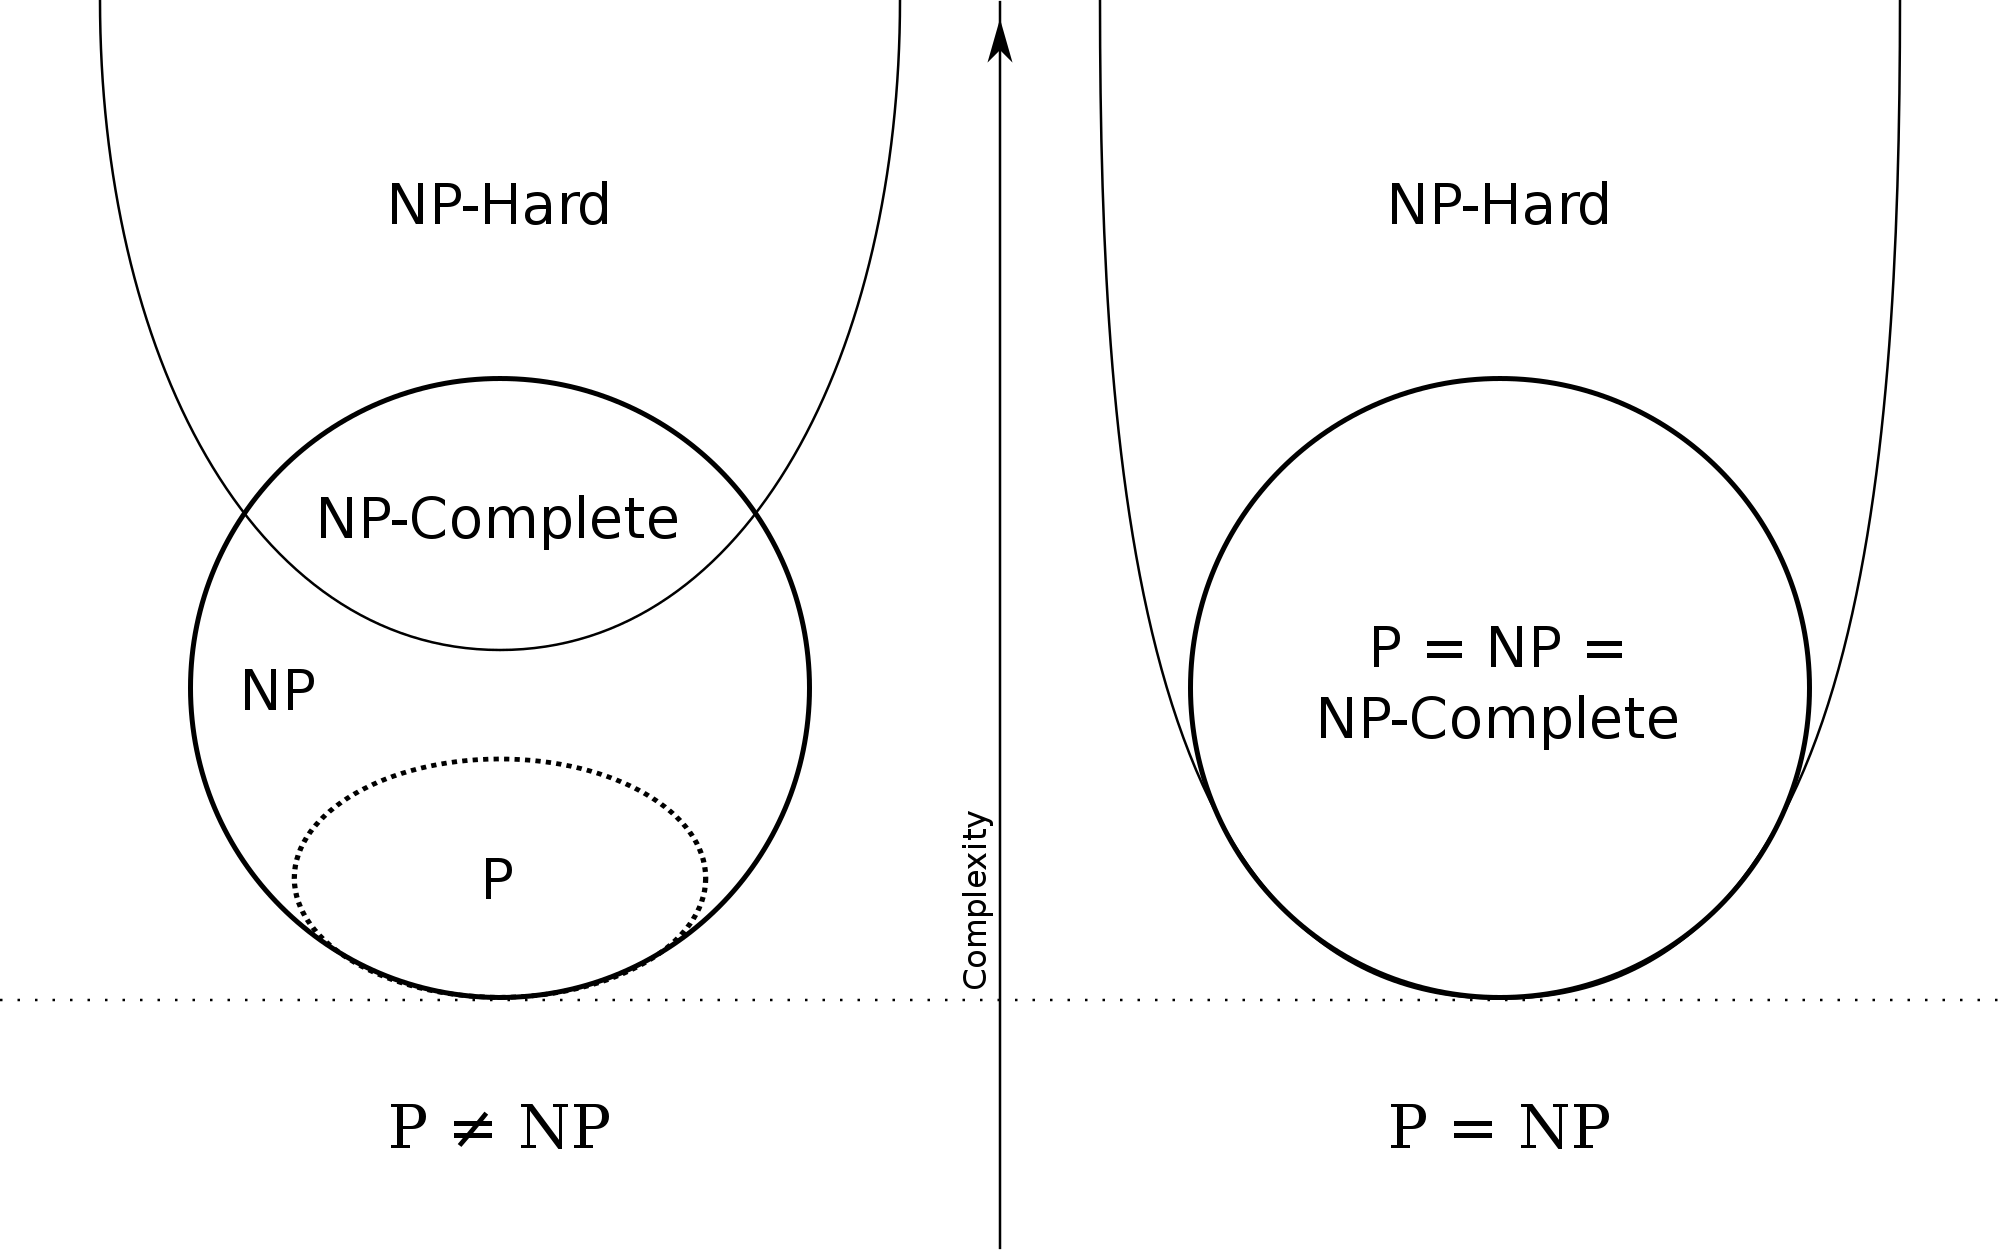
\includegraphics[scale=0.25]{complexity_classes.png} 
\centering
\caption{Complexity schema}
\end{figure}
\noindent Bearing in mind the complexity problem to face, the most reasonable solution is to solve the problem approximatively. The technique I used to generate the possible hamiltonian cycles is a genetic algorithm, while the choice of the shortest hamiltonian cycle is done by the \textit{simulated annealing} algorithm.

\section{Literature review}

\section{Algorithms and techniques} \label{algorithms}
In this section we provide a brief overview of all the techniques and aglorithms exploited. They are: Simualted Annealing, Metropolis algorithm and Genetic algorithm.

\subsection{Simulated annealing}
Simulated annealing (SA) is a technique that mimic the behaviour of heated materials slowly cooled down in metallurgy, this process decreases the impurity and increases the size of the crystals meaning that allows materials to reach the state that minimizes the energy. It is a technique to approximate the global optimal solution when the solutions is to be searched in an enormous space. SA is a metaheuristic meaning that it is not a probelm-specific stochastic heuristic. As every metaheuristic algorithm it relies on two principles \textit{intensitification} and \textit{diversification}, indeed, the algorithm intensifies the search near different possible optimal solutions.
SA is very useful since it does not require any prior information, other than the cost, indeed it just supposes that states (hamiltonian cycles in our case) are distributed accordingly to the Bolzmann distribution:
\begin{equation}
e^{- \beta (cost(state))}
\end{equation}
The Boltzmann distribution is suitable to model the TSP problem since it is most unbiased distribution among all the possible distributions. The undiasedness derives from the maximization of the Shannon entropy, given the cost. [METTI UNA CITAZIONE]\\
The underlying assumption of simulated annealing is that the optimal states are the states with the lowest cost, and they are reached as the temperature decreases.
he temperature $T$ is the inverse of $\beta$ ($T = \frac{1}{\beta}$), therefore we start with low values of $\beta$ (high temperature) and as the simulation proceeds we increase the values of $\beta$, thus mimicking the decrease in temperature.
The only other information needed is the cost function. For this specific application the cost function is the sum of euclidean distances between the cities in the cycle. The coordinate of a city $(x,y)$ are expressed in longitude and latitude.\\
In the following we provide a schematic overview of the simulated annealing implemented.

\begin{algorithm}[H]
    \begin{algorithmic}[1]
      \Function{simulated annealing}{\textbf{betas},number of simulations}
        \State s $\leftarrow$ generate starting state with the genetic algorithm
         \For {b in \textbf{betas}}
         	\For{n in 1,.., number of simulations}
         	 \State ns $\leftarrow$ generate a new state with the genetic algorithm starting from s
         	\State ns $\leftarrow$ METROPOLIS(s,ns,$\beta$)
         	\EndFor
        \EndFor
        \State return ns
       \EndFunction
\end{algorithmic}
\end{algorithm}

\noindent where \textbf{betas} is a set of the values of $\beta$. \\ 
The code executes all the procedures using a vectorial implementation to speed up the computation.

\subsection{Metropolis algorithm}
Metropolis is a Markov Chain Monte Carlo (MCMC) algorithm used to generate values $X_n$ from a finite set of values $S$ accordingly to a target probability distribution $\pi$.  \\
An homogeneous and finite Markov chain with state space $S$, transition matrix $P$ and initial distribution $\mu$ is a sequence of random variables $\{ X_n \}_{n \in N}$ such that
\begin{enumerate}
\item $\forall i \in S \, Pr(X_0=i)= \mu(i)$ 
\item $\forall n > 0 \; \forall i_n,...,i_0 \,  Pr(X_{n+1} = j | X_n = i_n,..., X_0=i_0) = Pr(X_{n+1} = j | X_n = i)$
\item $\forall n > 0 \, Pr(X_{n+1} = j | X_n = i) = p(i,j) $
\end{enumerate}
Metropolis algorithm is designed in such a way that it is very likely to move from a state with lower probability from a state with higher probability. \\
The following algorithm describes the metropolis algorithm when the target distribution is $\pi(\text{state}) = e^{- \beta \, \text{cost(state)}}$ and $S$ is the set of all possible hamiltonian cycles having fixed their length. In the following we suppose to have generated two hamiltonian cycles (i.e states) old\_state, new\_state and we want to understand if new\_state can come from $\pi$. If new\_state is likely to be a sample of $\pi$ we use it as new state otherwise we keep old\_state as the current state.

\begin{algorithm}[H]
    \begin{algorithmic}[1]
      \Function{metropolis}{old\_state, new\_state, $\beta$}
      	\If {cost(new\_state) $<$ cost(new\_state)}
      	\State return new\_state
      	\EndIf
        \State threshold $\leftarrow$ unif[0,1]
        \State p  $\leftarrow min\{1,e^{- \beta (\text{cost(new\_state}) - \text{cost(old\_state}))} \}$ 
        \If {p $>$ threshold}
        	\State return new\_state
        \Else
        	\State return old\_state
        \EndIf
       \EndFunction
\end{algorithmic}
\end{algorithm}
\noindent
\subsubsection{Properties of metropolis algorithm}
We can model the generation of new hamiltonian cycles using a undirected and connected graph $G = (S,E)$ whose set of states $S$ contains all the possible hamiltonian cycles and $E$ contains the transition probability from an hamiltonian cycle to another one. Given the graph, we can define the transition matrix $P=p(i,j)]_{i,j\in S}$ as
\begin{equation}
p(i,j) =  \begin{cases} 
	0\, & \mbox{if } \{i,j\} \notin E  \\ 
	\frac{1}{d_i} \min\{1,\frac{\pi(j)}{\pi(i)}\} & \mbox{if }  \{i,j\} \in E \;,\, i \neq j\\
	1-\frac{1}{d_i} \sum_{l \in adj(i)} \min\{1,\frac{\pi(l)}{\pi(i)}\}  & \mbox{if }  i = j 
\end{cases}
\end{equation}
Since G is a connected graph, the $P$ is irriducible meaning that $\forall i,j \in S \, p^n(i,j) > 0$, where $p^n(i,j)$ means that exist a path from $i$ to $j$ of length $n$.\\
It can also be proved that $P$ is aperiodic \cite{metropolis}. By aperidoicity we mean each node of the graph has a loop. More formally, th graph $G$ is aperiodic if $\forall i \in S, \,d(i)  = 1$ where
\begin{equation}
d(i) = mcd \{n \in N | \, \text{exist a cycle from i to i of length} \, n\}
\end{equation}
Metropolis algorithm defines a probability distributin $\pi$ that is a reversible distribution, meaning that
\begin{equation}
	\pi(i)p(i,j) = \pi(j)p(j,i) \;\; \forall i,j \in S
\end{equation}
This is a key feature of the algorithm since a reversible distribution $\pi$ is also a stationary distribution $\pi'P=\pi'$. This condition holds by the following theorem
\begin{theorem}
If a probability distribution $\pi$ is a reversible distribution for a markov chain $ \{X_n\} $, then it is also a stationary distribution.
\end{theorem}

\begin{proof}
$ (\pi'P)_j = \sum_{i \in S} \pi(i)p(i,j) = \sum_{i \in S} \pi(j)p(j,i) = \pi(j) $ 
\end{proof}
\noindent If this distribution was unique than we are certain to correctly generate the data accordingly to the target distribution. The stationary distibution is unique if the transition matrix is primitive as stated by the follwing theorem.
\begin{theorem}
Let $\{X_n\}$ be a markov chain with a primitive (i.e. irreducible and aperiodic) transition matrix on a finite set, then  there exist only one stationary distribution and it as also the limit distribution $\lim_{n \to \infty} p^n(i,j) = \pi(j)\,  \forall i \in S$
\end{theorem}
\noindent Since $P$ is primitive, it is enough to compute the limit distribution to find the unique stationary distribution. \\
The stationary distribution can be approximated in a logarithmic number of iterations starting from any distribution. Therefore to sample hamiltonian cycle from the stationary distribution is enough to let the simulation go on for a suitable number of iterations \cite{mcalgorithm}. \\

\subsection{Genetic algorithm}
Genetic algorithms are a widespread clarclengthss of algorithms that mimic nature. Indeed there are three fundamental operations they perform to generate new states (hamiltonian cycles in our case), each operation is inspired by the theory of evolution by C. Darwin. \\
Among a specie, evolution selects the fittest individuals and therefore the algorithm will chose the fittest (i.e shortest) hamiltonian cycles. \\
\begin{algorithm}[H]
    \begin{algorithmic}[1]
      \Function{selection}{\textbf{population},n\_paths}
        \State n\_parents $\leftarrow$ unif[2,n\_paths/2]
        \State order the population by fitness
        \State \textbf{fittest\_subpopulation} $\leftarrow$ extract n\_parents in order from the sorted population
        \State return \textbf{fittest\_subpopulation}
       \EndFunction
\end{algorithmic}
\end{algorithm}
\noindent The breeding of the fittest individuals produces new individuals that inherits traits from the parents, therefore in the crossbreeding phase we mix some subsection of the fittest hamiltonian cycles. \\
\begin{figure}[H]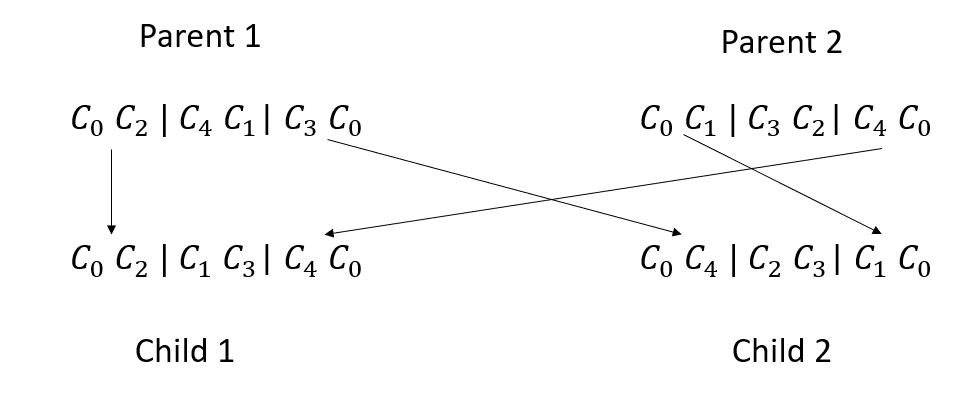
\includegraphics[scale=0.5]{crossbreeding.png} 
\centering
\caption{Crossbreeding schema}
\end{figure}

\noindent As random mutations can occur in nature but they are not so likely to occur, the algorithms swaps two cities with a fixed and low probability. The mutation probability should be low since otherwise if can disrupt the optimal subsequence of the cycle inherited. \\


\begin{algorithm}[H]
    \begin{algorithmic}[1]
      \Function{mutate}{\textbf{new\_population}, p}
      \For {path in \textbf{new\_population}}
        \State test $\leftarrow$ unif[0,1]
        \If {test $<$ p}
        	\State choose position1 randomly among unif[0,length of cycles-1)
  			\State choose position2 randomly among unif[0,length of cycles-1)
  			\State swap the cities in position1 and position2
        \EndIf
       \EndFor
        \State return \textbf{new\_population}
       \EndFunction
\end{algorithmic}
\end{algorithm}
\noindent To easily apply all the operations, a function was created.

\begin{algorithm}[H]
    \begin{algorithmic}[1]
      \Function{evolve}{\textbf{population}}
        \State \textbf{fittest\_population} $\leftarrow$ SELECT(\textbf{population})
        \State \textbf{new\_population} $\leftarrow$ CROSSBREED(\textbf{fittest\_population})
       \State \textbf{population} $\leftarrow$ MUTATE(\textbf{new\_population})
       \EndFunction
\end{algorithmic}
\end{algorithm}

\noindent There are many possible implementations of the basic operations performed by a genetic algorithm. Therefore I deicde to implement the from scratch.

\section{Application} 
The project consists in implementing the all the methods described in the section \ref{algorithms}.
We want to apply the algorithm to find the best cycle among some cities of northern Italy.
In this section we first provide the reader with the application of the previous methodologies to the problem. 

\subsection{Distance}
To realistically model the routes that connect important cities in northern Italy euclidean distance is a suitable measure since it approximates well the route of the highways
METTI UN' IMMAGINE

\subsection{Dataset}
The dataset consists in some provincial captial of norther Italy: \textit{Varese, Novara, Torino, Genova, Milano, Como, Bergamo, Brescia, Cremona, Lecco, Lodi, Mantova, Monza, Pavia, Sondrio, Verona, Vicenza, Padova, Venezia, Firenze, Pisa}. \\
The coordinates in terms of latitude and longitude were downloaded using a python library as follows:


\begin{figure}[H]
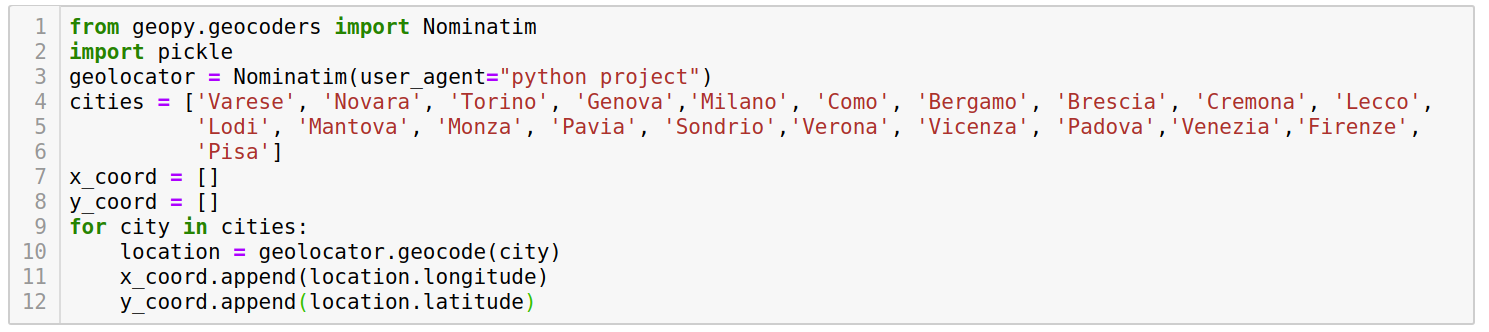
\includegraphics[scale=0.42]{download_dataset.png} 
\centering
\caption{Python code to download the coordinates of the cities}
\end{figure}

\subsection{Software used}
The objective of this simulation is to show compare the optimal solutions of the TSP computed by the appromated algorithm and by the exact algorithm.
The exact solution of the TSP is not feasible when the number of cities grows too much therefore we compute exact solutions as long as it is feasible. \\
We provide an schematic description of the experiement run. 
\begin{algorithm}[H]
    \begin{algorithmic}[1]
      \Function{Experiment}{all\_cities}
       \For {i in 1,..., n\_cities}
       	\State  cities $\leftarrow$ all\_cities[0:i]
       	\For {for all threads}
       		\State run simluted annealing in parallel
       	\EndFor 
       	\State extract the best solution among the solutions computed by the threads
       	\If{i < feasibility\_threshold}
       		\State compute the exact solution
       	\EndIf
       	\State compare the results by plotting them
       \EndFor
       \EndFunction
\end{algorithmic}
\end{algorithm}

\noindent In this section we provide the python code that runs the simulation\\
\\
\begin{figure}[H]
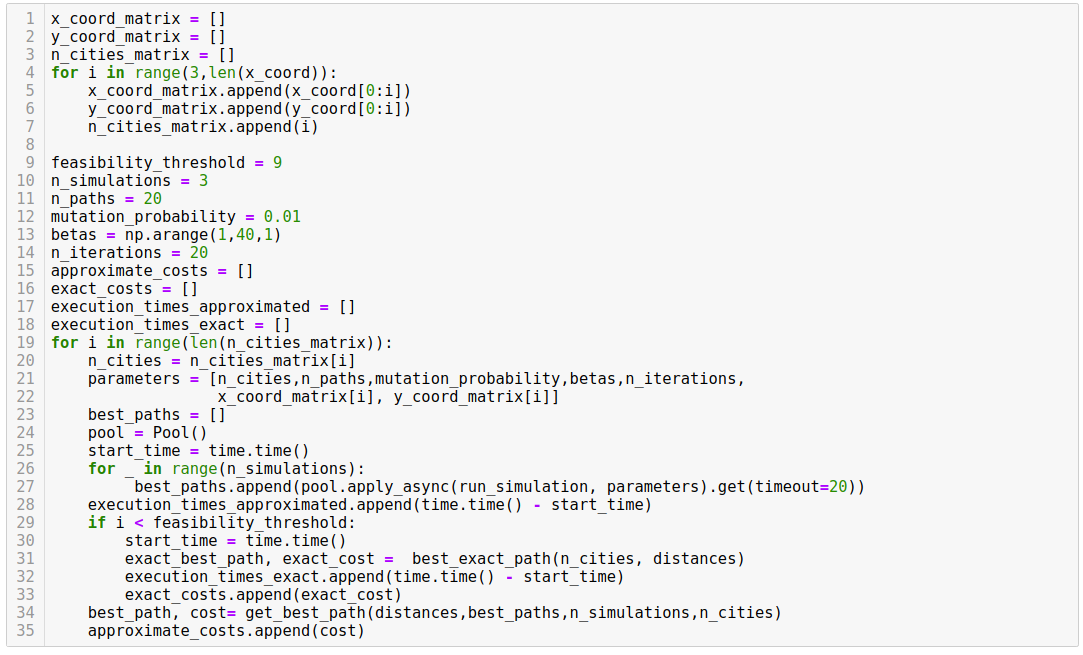
\includegraphics[scale=0.5]{simulation.png} 
\centering
\caption{Python code of the experiment}
\end{figure}

\begin{algorithm}[H]
    \begin{algorithmic}[1]
      \Function{run\_simulation}{\textbf{betas}, n\_iterations}
      \State generate a starting population
       \For {beta in betas}
       		\For {i in 1,...,n\_iterations}
       		\State EVOLVE the population
       		\State obtain the new state by metropolis algorithm
       	\EndFor 
       \EndFor
       \State return the shortest cycle
       \EndFunction
\end{algorithmic}
\end{algorithm}



\begin{figure}[H]
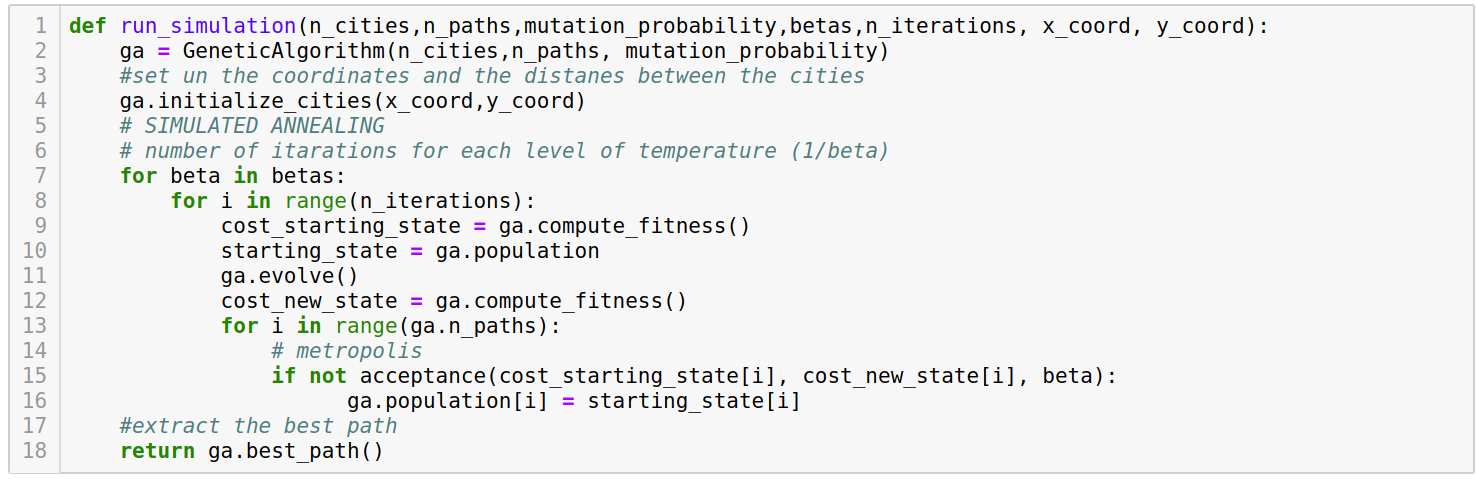
\includegraphics[scale=0.38]{run_simulation.png} 
\centering
\caption{Python code of a simulation}
\end{figure}
\noindent This method executes the simulated annealing. Indeed, we generate a starting population, we evolve it and accept or reject it with the metropolis algorithm.

\noindent To be able to control and modify the code as i wish, all the algorithm described were implemented from scratch exploiting just some support libraries as \textit{numpy}, \textit{pyplot}, etc.

\section{Results}
In this section we compare the Simulated annealing with the exact algorithm to solve the TSP problem. As expected the computational time required to compute an exact solutions becomes too big as the length of the cycles increases. It is more efficient that the simulated annealing for small length of the cycles, since it perform faster and fewer operations. On the coutrary, the execution time of the SImulated Annealing is almost independent from the length of the cycles. The slight variations and the peaks in the plot may be dued to the scheduling of the operating system and its scheduler and the multithreading.
\begin{figure}[H]
\begin{adjustwidth}{-4em}{-4em}

     \subfloat{%
       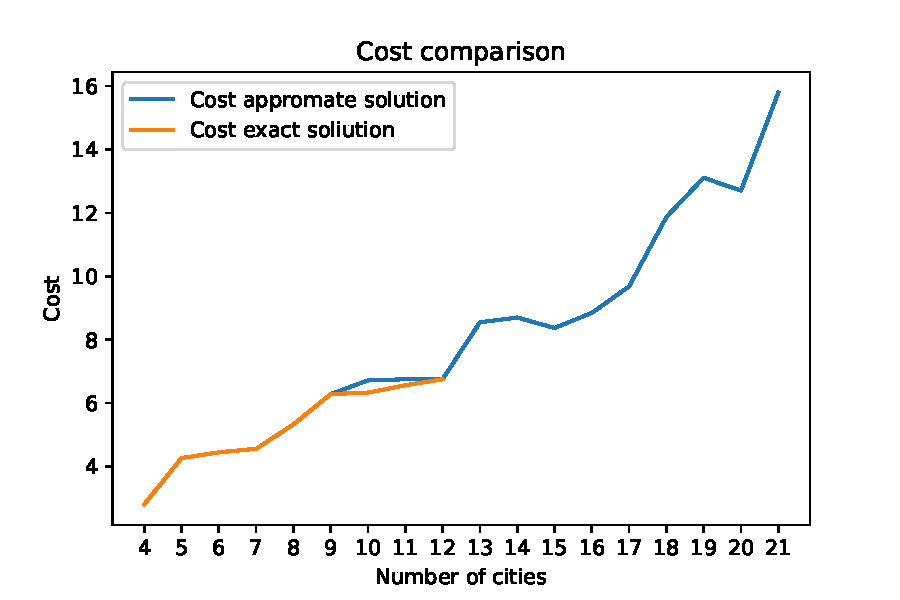
\includegraphics[width=0.60\textwidth]{../Cost_comparison.pdf} 
     }
     \hfill
     \subfloat{%
       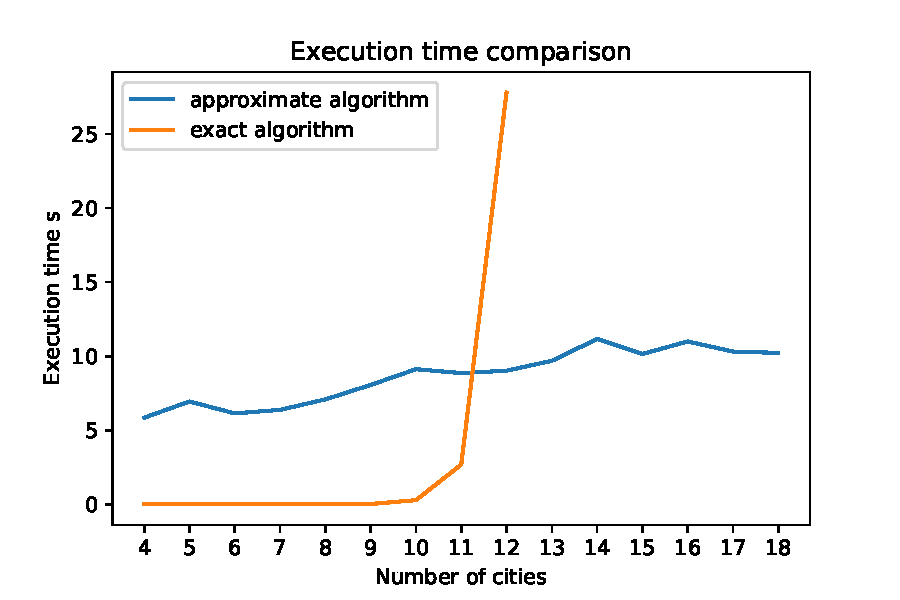
\includegraphics[width=0.60\textwidth]{../Time_comparison.pdf} 
     }
     
     \caption{Comparison}
    \end{adjustwidth}
   \end{figure}
\noindent As the plot above shows, simulated annealing is capable of finding optimal or slightly suboptimal solutions. However, it is reasonable to expect that as the length of the cycles increases the optimal solutions of the simulated annealing gets further away from the very best optimal solution.\\
In the following we also plotted the shortest cycle computed by the simulated annealing when using all the possible cities. As starting point i choose provicial capital nearest to my home.
\begin{figure}[H]
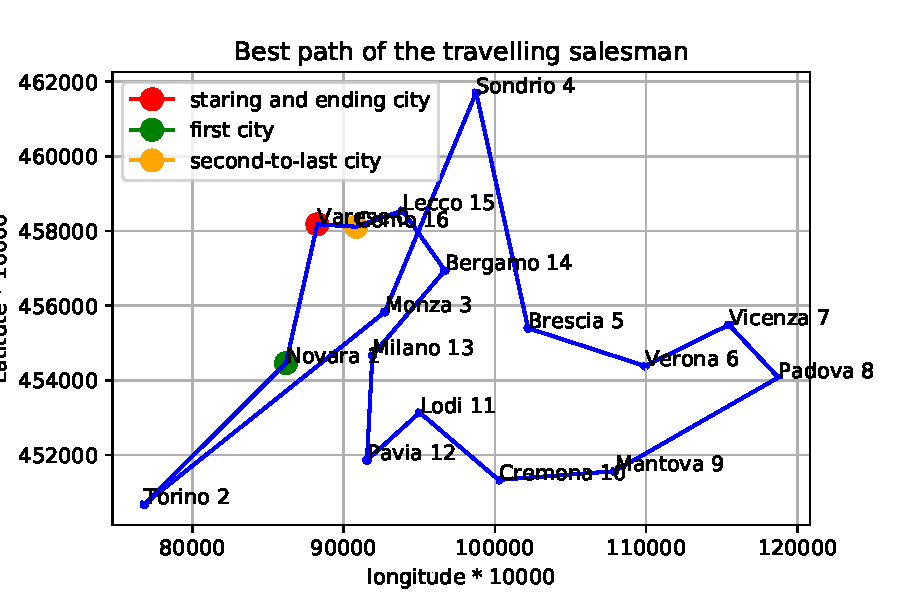
\includegraphics[scale=1]{../path.pdf} 
\centering
\caption{Optimal cycle starting from Varese}
\end{figure}

ighway\section{Conclusion}
Overall the simulated annealing and the genetic algorithm seem to have quite good performances. The cost function is almost always increasing and as far as it is possible to compare the simulated annealing finds very optimal cycle while keeping the execution time very low. \\
As far as execution time is concerned, the length of the cycles seems to have a very limited influnce on the overall execution time, indeed, it exhibits almost a constant behaviour. \\
As for the optimal cycle computed, for all of the cities the euclidean distance provides a suitable approximation of the routes of the highways present in northern Italy. However, this notion of distance does not take into account the TEMPO DI PERCORRENZA of the highways that can significantly change during the day and may not be correlated to significantly with the length of the highways.

\newpage

\begin{thebibliography}{9}

\bibitem{metropolis}
Oliver Catoni
\textit{Simulated annealing algorithms and Markov chains with rare transitions}, Séminaire de probabilités (Strasbourg), tome 33 (1999), p. 69-119.

\bibitem{mcalgorithm}
Marius Iosifescu
\textit{Finite markov process and their applications}, John Wiley \& Sons, 1980.

\bibitem{gaBraun}
Heinrich Braun
\textit{On solving the travelling salesman problems by genetic algoritms}

\bibitem{gareview}
P. LARRAÑAGA, C.M.H. KUIJPERS, R.H. MURGA, I. INZA and S. DIZDAREVIC
\textit{Genetic Algorithms for the Travelling Salesman Problem: A Review of Representations and Operators}, Artificial Intelligence Review 13: 129–170, 1999.

\bibitem{test}
https://upload.wikimedia.org/wikipedia/commons/thumb/a/a0/P\_np\_np-complete\_np-hard.svg/2000px-P\_np\_np-complete\_np-hard.svg.png

 
\end{thebibliography}

\end{document}